\documentclass[12pt,a4paper]{article}
\usepackage[utf8x]{inputenc}
\usepackage{ucs}
\usepackage[english,russian]{babel}
\usepackage[OT1]{fontenc}
\usepackage{amsmath}
\usepackage{amsfonts}
\usepackage{amssymb}
\usepackage{wasysym}
\usepackage{physics}
\usepackage{wrapfig}
\usepackage{mathrsfs}

%---------Схемы---------
\usepackage{circuitikz}
%-----------------------

%--------Графики--------
\usepackage{pgfplots}
%Чтобы хорошо работало
\pgfplotsset{compat=1.9}
%----------------------

\usepackage[left=2cm,right=2cm,top=2cm,bottom=2cm,includefoot,footskip=1.5cm]{geometry}

\usepackage{fancyhdr}
\pagestyle{fancy}

\usepackage[T1]{fontenc}
 
\usepackage{indentfirst}
%% Sets page size and margins
%\usepackage[dvips]{graphicx}
%\graphicspath{{noiseimages/}}
%\usepackage[colorinlistoftodos]{todonotes}
%\usepackage[colorlinks=true, allcolors=blue]{hyperref}

\rhead{\small Д.\,Павлов, А.\,Савко, МФТИ}
\lhead{Лабораторная работа №3.2.1}

\author{Дмитрий Павлов, 790 \\  Александр Савко, 790}
\title {\textbf{Сдвиг фаз в цепи переменного тока}}

\begin{document}
\maketitle
\newpage
\tableofcontents 

\newpage

\section{Вступление.}
    \subsection{Цель работы.}
        Исследование зависимости сдвига фаз между током и напряжением от сопротивления в $RC$- и в $RL-$цепи; определение добротности колебательного контура, при помощи полученной в работе зависимости сдвига фаз от частоты вблизи резонанса; оценка диапазона работы фазовращателя.
        
    \subsection{Оборудование.}
        \begin{itemize}
            \item Звуковой генератор (ЗГ);
            \item Двухканальный электронный осциллограф (ЭО);
            \item Магазин емкостей;
            \item Магазин сопротивлений;
            \item Эталонная катушка индуктивности;
            \item Резисторы;
            \item Мост переменного тока.
        \end{itemize}

    \subsection{Экспериментальная установка.}
        \begin{wrapfigure}{2}{0.6\linewidth}
        	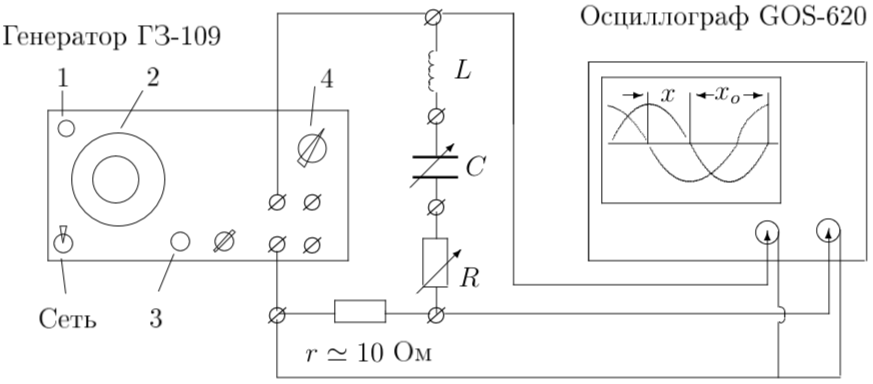
\includegraphics[width=\linewidth]{ris1.png}
        	\hspace{44pt}{Рисунок 1 -- Схема для исследования сдвига фаз между током и напряжением в цепи переменного тока.}
        	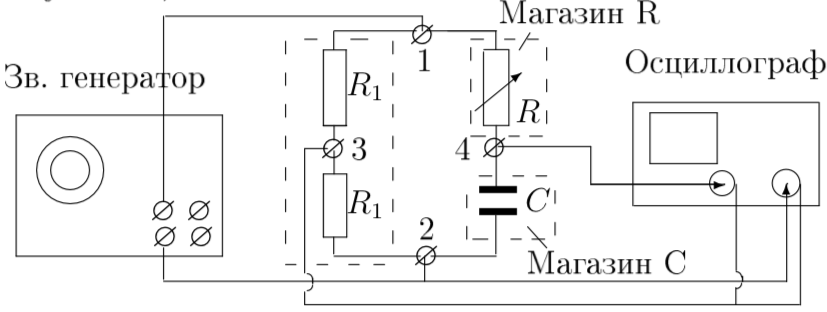
\includegraphics[width=\linewidth]{ris2.png}
        	\hspace{44pt}{Рисунок 2 -- Схема фазовращателя.}
        \end{wrapfigure}
        
        Схема для исследования сдвига фаз между током и напряжением в цепи переменного тока представлена на рис. 1. Эталонная катушка $L$, магазин емкостей $C$ и магазин сопротивлений $R$ соединены последовательно и через дополнительное сопротивление $r$ подключены к источнику синусоидального напряжения - звуковому генератору.
        
        Сигнал, пропорциональный току, снимается с сопротивления $r$, пропорциональный напряжению - с генератора. Оба сигнала подаются на универсальный осциллограф. Этот осциллограф имеет два канала вертикального отклонения, что позволяет одновременно наблюдать на экране два сигнала.
        
        Схема фазовращателя, изображенная на рис. 2, содержит два одинаковых резистора $R_1$, смонтированных на отдельной плате, магазин сопротивлений $R$ и магазин емкостей $C$.

\newpage
\section{Теоретическая часть.}
    \subsection{Общий случай.}
        Рассмотрим $RLC$-контур, подключённый к источнику внешней ЭДС, изменяющейся по гармоническому закону: $\mathscr{E} = \mathscr{E}_0\cos{(\Omega t)}$. 
        
        \begin{center}
            \begin{circuitikz} \draw 
                (0,0)   to[sV,l=$\mathscr{E}_0\cos{\Omega t}$] (0,3) 
                        to[C=$C$] (3,3)
                        to[american inductor=$L$] (3,0) 
                        to[generic=$R$] (0,0);
            \end{circuitikz}
        \end{center}
        
        Обозначим разность потенциалов на конденсаторе через $U_C$, а ток, текущий в контуре, через $I$. Сумма падений напряжения на элементах цепи равна ЭДС самоиндукции плюс ЭДС источника:
        \[
        RI + U_C = -L \frac{dI}{dt} + \mathscr{E}_0\cos{\Omega t}
        \]
        При решении линейного дифференциального уравнения получаем выражение:
        \[
        I_0\Big[R + i\Big(\Omega L - \frac{1}{\Omega C}\Big)\Big] = \mathscr{E}_0
        \]
        Величина, стоящая в скобках называется импедансом контура и обозначается $Z$
        \[
        Z = R + i\Big(\Omega L - \frac{1}{\Omega C}\Big)
        \]
        Представим импеданс $Z$ в показательной форме:
        \begin{equation}\label{eq:1} %\hspace{15}
            Z = |Z|e^{i\psi};   |Z| = \sqrt{R^2 + \Big(\Omega L - \frac{1}{\Omega C}\Big)^2}; \psi = \arctg{\frac{\Omega L - \frac{1}{\Omega C}}{R}}
        \end{equation}
        Итого, ток отстаёт от напряжения по фазе на величину $\psi$, определяемую отношением мнимой и действительной частей импеданса. Амплитуда колебаний обратно пропорциональна модулю импеданса $|Z|$.

    \subsection{Векторные диаграммы.}
        Рассмотрим несколько частных случаев.
        \begin{enumerate}
            \item К источнику синусоидального напряжения подключено только чисто активное сопротивление $R$. В этом случае из формул ($\ref{eq:1}$) следует, что $\psi$ = 0. Ток в активном сопротивлении совпадает по фазе с напряжением на нём.
            \item К источнику подключена только ёмкость $C$ (конденсатор без потерь). При этом $\psi = −\pi/2$. Ток опережает напряжение по фазе на $\pi/2$.
            \item К источнику подключена только катушка самоиндукции с индуктивностью $L$,активное сопротивление которой $R_L = 0$. При этом $\psi = \pi/2$. Ток в цепи отстаёт по фазе от напряжения на $\pi/2$.
            \item В общем случае, когда к источнику последовательно подключены резистор, конденсатор и катушка самоиндукции, сдвиг фазы между то- ком и входным напряжением лежит в пределах: $−\pi/2 < \psi < +\pi/2$.
        \end{enumerate}
        
        Построим векторную диаграмму напряжений для контура, изображённого на рис. В.6. К источнику переменного напряжения $\mathscr{E}_0\cos{\Omega t}$ последовательно подключены резистор $R$, катушка индуктивности $L$, действительная часть импеданса которой равна $r_L$, и ёмкость $C$. Четыре вольтметра измеряют напряжения на элементах цепи, амперметр измеряет ток.
        \begin{figure}[h!]
        	\begin{center}
        		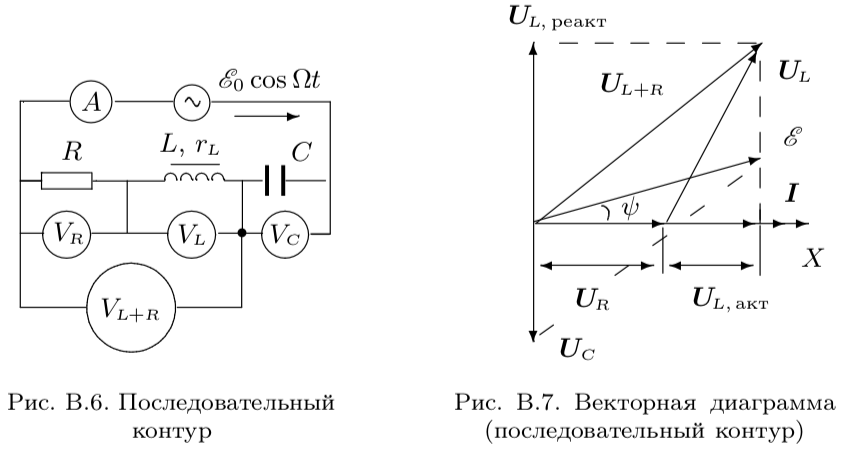
\includegraphics[width=0.8 \textwidth]{zero}\\
            	{\scriptsize
            	\begin{center}
            	\end{center}}
        	\end{center}
            \label{scheme1}
        \end{figure}
        
        Отложим вектор $I$ вдоль оси абсцисс (рис. В.7). Напряжение на резисторе совпадает по фазе с током, поэтому вектор $U_R$ также будет направлен вдоль оси абсцисс. Напряжение на конденсаторе (без потерь) отстаёт по фазе от тока на угол $\psi = \pi/2$, поэтому вектор $U_C$ направлен вниз вдоль оси ординат.Векторное равенство напряжений $U_{L+R} = U_L + U_R$ позволяет построить треугольник по трём сторонам. Сделаем две насечки: первую — радиусом, равным модулю вектора $U_{L+R}$ , из начала вектора $U_R$ (начала координат); вторую — радиусом, равным модулю вектора $U_L$, из конца вектора $U_R$. Точка пересечения насечек определяет положение векторов $U_{L+R}$ и $U_L$ на диаграмме. Сложив векторы $U_{L+R}$ и $U_C$, получим вектор входного напряжения на контуре. Угол $\psi$ показывает, каков сдвиг фаз между током и напряжением в цепи.
        
        Разложим теперь вектор $U_L$ по осям координат. Проекция $U_L$ на ось абсцисс позволяет определить $U_{L,\text{акт}}$  — напряжение на активной части импеданса катушки, а проекция на ось ординат даёт реактивную часть $U_{L,\text{реакт}}$. Поделив эти напряжения на ток $I$ , найдём действительную часть импеданса катушки $r_L$ и мнимую $\Omega L$.

\newpage
\section{Основная работа.}
    \subsection{Исследование зависимости сдвига фаз между током и напряжением от $R$ в $RC-$цепи.}
        Пользуясь схемой, изображенной на рис. 1, найдем зависимость сдвига фаз между током и напряжением от $R$ в $RC-$цепи. Для этого закоротим катушку индуктивности. На магазине емкости поставим емкость $C = 0.5$ мкФ, $\nu = 1$ кГц.
        
        Рассчитаем реактивное сопротивление цепи по формуле: $X_1 = 1/(\Omega C) = 1/(2 \pi \nu C)$. Где $\Omega = 2 \pi \nu$ - циклическая частота.
        
        \[
        X_1 = \frac{1}{\Omega C} = \frac{1}{2 \pi \nu C} = \frac{1}{2 \pi \cdot 1000 \text{Гц} \cdot 0.5 \text{мкФ}} = 318.3 \text{Ом}.
        \]
        
        Увеличивая сопротивление $R$ от нуля до $10 \cdot X_1$, проведем измерения сдвига фаз $\psi$.
        
        \begin{table}[!h]
        \begin{flushleft}%\hspace{80}
       		\textbf{Таблица 1} -- Сдвиг фаз в $RC-$контуре в зависимости от  $R$.\\
        \end{flushleft}
            \begin{center}
                \begin{tabular}{ | l | l | l | l |}
                    \hline
                    $R$, Ом &   $x$, см &  $x_0$, см &   $\psi$  \\
                    \hline
                    0   &   2.5 &   5   &   0.5$\pi$\\
                    200 &   1.6 &   5   &   0.32$\pi$\\
                    400 &   1.2 &   4.4 &   0.27$\pi$\\
                    600 &   0.4 &   4.5 &   0.09$\pi$\\
                    900 &   0.6 &   5   &   0.12$\pi$\\
                    1200&   0.2 &   4.5 &   0.04$\pi$\\
                    \hline                
                \end{tabular}
            \end{center}
        \end{table}
            
    \subsection{Исследование зависимости сдвига фаз между током и напряжением от $R$ в $RL-$цепи.}
        Пользуясь схемой, изображенной на рис. 1, найдем зависимость сдвига фаз между током и напряжением от $R$ в $RL-$цепи. Для этого закоротим магазин емкостей. На катушке поставим индуктивность $L = 50$ мГн, $\nu = 1$ кГц.
        
        Рассчитаем реактивное сопротивление цепи по формуле: $X_2 = \Omega L = 2 \pi \nu C$. 
        
        \[
        X_2 = \Omega L = 2 \pi \nu L = 2 \pi \cdot 1000 \text{Гц}\cdot 50\text{Гн} = 314 \text{Ом}.
        \]
        
        Увеличивая сопротивление $R$ от нуля до $10 \cdot X_2$, проведем измерения сдвига фаз $\psi$.
        
        \begin{table}[!h]
        \begin{flushleft}%\hspace{80}
       		\textbf{Таблица 2} -- Сдвиг фаз в $RL-$контуре в зависимости от  $R$.\\
        \end{flushleft}
            \begin{center}
                \begin{tabular}{ | l | l | l | l |}
                    \hline
                    $R$, Ом &   $x$, см &  $x_0$, см&   $\psi$      \\
                    \hline
                    0       &   2.2     &   4.9     &   0.45$\pi$   \\
                    200     &   1.4     &   4.9     &   0.29$\pi$   \\
                    600     &   0.6     &   4.9     &   0.12$\pi$   \\
                    900     &   0.4     &   4.9     &   0.08$\pi$  \\
                    1200    &   0.2     &   4.9     &   0.04$\pi$  \\
                    \hline                
                \end{tabular}
            \end{center}
        \end{table}
        
    \subsection{Исследование зависимости сдвига фаз между током и напряжением от частоты в $RLC$-контуре.}
        В цепи, изображенной на рис. 1, Установим значения $R = 0$, $L = 50$ мГн, $C = 0.5$ мкФ. Рассчитаем резонансную частоту по формуле: $\nu = 1/(2 \pi \sqrt{LC})$.
        
        \[
        \nu = \frac{1}{(2 \pi \sqrt{LC})} = \frac{1}{2 \pi \sqrt{50\text{мГн} \cdot 0.5 \text{мкФ}}} = 1006 \text{Гц}.
        \]
        
        Снимем зависимость сдвига фаз от частоты. Для этого:
        \begin{itemize}
            \item Подберем частоту ЗГ, чтобы получить резонанс в цепи. При резонансе $\psi = 0$, и нулевые значения двух синусоид должны совместиться, а при равенстве амплитуд синусоиды полностью совпадают.
            \[
            \nu_{\text{эксп}} = 1020 \text{Гц}.
            \]
            \item Оценим по картинке на экране ЭО диапазон измерения частоты, в котором сдвиг фазы меняется от $\pi/3$ до $-\pi/3$.
            \item Снимем зависимость сдвига фаз от частоты в этом диапазоне, меняя частоту в обе стороны от резонансного значения. С изменением частоты меняется расстояние $x_0$, которое занимает половина периода синусоиды, поэтому каждый раз фиксируем отношение $x/x_0$.
            
            \begin{table}[!h]
            \begin{flushleft}%\hspace{20}
           		\textbf{Таблица 3} -- Сдвиг фаз в $RLC-$контуре в зависимости от частоты при $R = 0$ Ом.\\
            \end{flushleft}
                \begin{center}
                    \begin{tabular}{ | l | l | l | l | l | l | l | l |}
                        \hline
                        $\nu$, Гц   &   $x$, см &  $x_0$, см&   $\psi$  &   $\nu$, Гц   &   $x$, см &  $x_0$, см&   $\psi$  \\
                        \hline
                        910     &   1.6 &   5.3 &   0.3$\pi$    &   1020    &   0   &   4.8 &   0           \\
                        930     &   1.5 &   5   &   0.3$\pi$    &   1040    &   0.5 &   4.8 &   0.1$\pi$    \\
                        950     &   1.2 &   5   &   0.24$\pi$   &   1060    &   0.8 &   4.7 &   0.17$\pi$   \\
                        970     &   0.9 &   5   &   0.18$\pi$   &   1090    &   1   &   4.6 &   0.22$\pi$   \\
                        990     &   0.6 &   5   &   0.12$\pi$   &   1100    &   1.2 &   4.5 &   0.27$\pi$   \\
                        1000    &   0.3 &   4.8 &   0.06$\pi$   &   1120    &   1.3 &   4.4 &   0.3$\pi$    \\
                        \hline         
                    \end{tabular}
                \end{center}
            \end{table}   
            \item Повторим измерения сдвига фаз для сопротивления $R = 100$ Ом.
            
            \begin{table}[!h]
            \begin{flushleft}%\hspace{20}
           		\textbf{Таблица 4} --  Сдвиг фаз в $RLC-$контуре в зависимости от частоты при $R = 100$ Ом.\\
            \end{flushleft}
                \begin{center}
                    \begin{tabular}{ | l | l | l | l | l | l | l | l |}
                        \hline
                        $\nu$, Гц   &   $x$, см &  $x_0$, см&   $\psi$  &   $\nu$, Гц   &   $x$, см &  $x_0$, см    &   $\psi$  \\
                        \hline
                        900     &   0.8 &   5.2 &   0.15$\pi$   &   1020    &   0   &   4.8 &   0           \\
                        920     &   0.6 &   5   &   0.12$\pi$   &   1040    &   0.2 &   4.8 &   0.04$\pi$  \\
                        940     &   0.4 &   5   &   0.08$\pi$   &   1060    &   0.4 &   4.7 &   0.09$\pi$  \\
                        960     &   0.3 &   5   &   0.06$\pi$   &   1090    &   0.5 &   4.6 &   0.11$\pi$   \\
                        980     &   0.2 &   4.9 &   0.04$\pi$   &   1100    &   0.6 &   4.5 &   0.13$\pi$   \\
                        1000    &   0   &   4.8 &   0           &   1120    &   0.6 &   4.5 &   0.08$\pi$   \\
                        \hline         
                    \end{tabular}
                \end{center}
            \end{table}
        \end{itemize}
    
        \begin{table}[!h]
            \begin{flushleft}%\hspace{87}
           		\textbf{Таблица 5} - Проверка приборов с помощью моста E7-8.
            \end{flushleft}
            \begin{center}
                \begin{tabular}{ | l | l | l |}
                    \hline
                    Значение        &   Номинальное, Ом &   Реальное, Ом \\
                    \hline
                    r               &   12.4            &   12.43    \\
                    $R_\text{кат}$  &   31.5            &   32.77    \\
                    \hline                
                \end{tabular}
            \end{center}
        \end{table}

    \subsection{Исследование работы фазовращателя.}
        Необходимо найти сопротивление $R$, при котором сдвиг фаз равен $\pi/2$. Соберем схему, изображенную на рис. 2, и установим $C = 0.5$мкФ, $\nu = 1$ кГц. При $R = 3800$ Ом сдвиг фаз равен $\pi/2$.
        
    \newpage
    
    \section{Обработка результатов.}
        \subsection{$RC$-цепь.}
            Для $RC$-цепи построим график $\psi = f(R+r)$, где $R$ - сопротивление, выставленное на магазине сопротивлений, $r$ - сопротивление резистора, включенного в цепь. Из графика определим сопротивление $R$ для $\psi$ = $\pi/2$.
                \begin{center}
                    \begin{tikzpicture}
                        \begin{axis}[
                            title = Сдвиг фаз в $RC$-цепи в зависимости от сопротивления $R$,
                            grid = major,
                            height = 0.25\paperheight, 
                	        width = 0.8\paperwidth,
            	            xlabel = {$R$, Ом},
            	            ylabel = {$\psi$, $\pi$},
            	            xmin = -50,
            	            xmax = 1250,
            	            ymin = -0.05
                        ]
                        \legend{ 
            	            ,$y = -3.54\cdot10^{-4}x+0.419$
                        };
                        \addplot[only marks,
                            error bars/.cd,
                            x dir=both, x explicit,
                            y dir=both, y explicit,] 
                            table [y error=error] {
                                x       y       error
                                0       0.5     0.05
                                200     0.32    0.05
                                400     0.27    0.05
                                600     0.09    0.05
                                900     0.12    0.05
                                1200    0.04    0.05
                            };
                        \addplot[draw = red]coordinates {
            	            (0,0.419) (1183,0)
                        };
                        \end{axis}
                    \end{tikzpicture}    
                \end{center}
                
                По графику определим сопротивление $R$, для $\psi = \pi/2$. $R =$, при этом рассчитанное значение: $R= 314$ Ом. 
                
                Построим график $tg{\psi} = f(\frac{1}{\omega R_\sum C})$, где $R_\sum = R + r$. Построим также теоретический график (пунктир).
                \begin{center}
                    \begin{tikzpicture}
                        \begin{axis}[
                            title = Сдвиг фаз в $RC$-цепи в зависимости от $RC\Omega$,
                            grid = major,
                            height = 0.25\paperheight, 
                	        width = 0.8\paperwidth,
            	            xlabel = {$RC\Omega$, безразмерная},
            	            ylabel = {$\tg{\psi}$},
            	            xmin = -0.05,
            	            xmax = 1.55,
            	            ymin = -0.05
                        ]
                        \legend{ 
            	            ,$y = -0.349x+0.526$
                        };
                        \addplot[only marks,
                            error bars/.cd,
                            x dir=both, x explicit,
                            y dir=both, y explicit,] 
                            table [y error=error] {
                                x       y       error
                                0.04    0.5     0.05
                                0.59    0.32    0.05
                                0.91    0.27    0.05
                                1.09    0.09    0.05
                                1.24    0.12    0.05
                                1.31    0.04    0.05
                            };
                        \addplot[draw = red] coordinates {
            	            (0,0.526) (1.507,0)
                        };
                        \addplot[dashed, draw = blue] coordinates {
                            (0,0.501) (1.530,0)
                        };
                        \end{axis}
                    \end{tikzpicture}    
                \end{center}
        \newpage
        \subsection{$RL$-цепь.}
            Для $RL$-цепи построим график $\psi = f(R+r+R_L)$, где $R_L$ - сопротивление, выставленное катушки индуктивности. Из графика определим сопротивление $R$ для $\psi$ = $\pi/2$.
            \begin{center}
                \begin{tikzpicture}
                    \begin{axis}[
                        title = Сдвиг фаз в $RL$-цепи в зависимости от сопротивления $R$ ,
                        grid = major,
                        height = 0.25\paperheight, 
            	        width = 0.8\paperwidth,
        	            xlabel = {$R$, Ом},
        	            ylabel = {$\psi$, $\pi$},
        	            xmin = -50,
        	            xmax = 1250,
        	            ymin = -0.05
                    ]
                    \legend{ 
        	            ,$y = -3.16\cdot10^{-4}x+0.371$
                    };
                    \addplot[only marks,
                        error bars/.cd,
                        x dir=both, x explicit,
                        y dir=both, y explicit,] 
                        table [y error=error] {
                            x       y       error
                            0       0.45    0.05
                            200     0.29    0.05
                            400     0.20    0.05
                            600     0.12    0.05
                            900     0.08    0.05
                            1200    0.04    0.05
                        };
                    \addplot[draw = red] coordinates {
        	            (0,0.371) (1174,0)
                    };
                    \end{axis}
                \end{tikzpicture}    
            \end{center}
        
            По графику определим сопротивление $R$, для $\psi = \pi/2$. $R =$, при этом рассчитанное значение: $R=310$ Ом. 
            
            Построим график $\tg{\psi} = f(\frac{\omega L}{R_1})$, где $R_1 = R + r + R_L$. Построим также теоретический график (пунктир).
            \begin{center}
                \begin{tikzpicture}
                    \begin{axis}[
                        title = Сдвиг фаз в $RL$-цепи в зависимости от $R/L\Omega$,
                        grid = major,
                        height = 0.25\paperheight, 
            	        width = 0.8\paperwidth,
        	            xlabel = {$R/L\Omega$, безразмерная},
        	            ylabel = {$\tg{\psi}$},
        	            xmax = 1.55,
        	            xmin = 0,
        	            ymin = 0
                    ]
                    \legend{ 
        	            ,$y = -0.339x+0.506$
                    };
                    \addplot[only marks,
                        error bars/.cd,
                        x dir=both, x explicit,
                        y dir=both, y explicit,] 
                        table [y error=error] {
                            x       y       error
                            0.14    0.45    0.05
                            0.66    0.29    0.05
                            0.96    0.20    0.05
                            1.12    0.12    0.05
                            1.25    0.08    0.05
                            1.32    0.04    0.05
                        };
                    \addplot[draw = red] coordinates {
                        (0,0.506) (1.492,0)
                    };
                    \addplot[dashed, draw = blue] coordinates {
                        (0,0.476) (1.508,0)
                    };
                    \end{axis}
                \end{tikzpicture}    
            \end{center}
            
        \newpage
        \subsection{Поиск добротности контура.}
        Найдем добротность колебательного контура при $R = 0 \Omega$ и $R = 100 \Omega$. Для этого измерим $\Delta \nu$ при сдвиге фаз $\psi = \pi/4$. Тогда $Q = \nu_0/(2\Delta \nu)$.
        
            \begin{tikzpicture}
                \begin{axis}[
                    title = {$R = 0$},
                    grid = major,
                    height = 0.25\paperheight, 
        	        width = 0.33\paperwidth,
    	            xlabel = {$\nu/\nu_0$},
    	            ylabel = {$\psi$, $\pi$},
    	            xmax = 1.12,
    	            xmin = 0.88,
    	            ymin = -0.05
                ]
                \addplot[
                    smooth,
                    error bars/.cd,
                    x dir=both, x explicit,
                    y dir=both, y explicit,] 
                    table [y error=error] {
                        x       y       error
                        0.905   0.30    0.02
                        0.924   0.30    0.02
                        0.944   0.24    0.02
                        0.964   0.18    0.02
                        0.984   0.12    0.02
                        0.994   0.06    0.02
                        1.014   0.00    0.02
                        1.034   0.10    0.02
                        1.054   0.17    0.02
                        1.083   0.22    0.02
                        1.093   0.27    0.02
                        1.113   0.30    0.02
                    };
                 \end{axis}
            \end{tikzpicture}    
            \begin{tikzpicture}
                \begin{axis}[
                    title = {$R = 100$},
                    grid = major,
                    height = 0.25\paperheight, 
        	        width = 0.33\paperwidth,
    	            xlabel = {$\nu/\nu_0$},
    	            ylabel = {$\psi$, $\pi$},
    	            xmax = 1.12,
    	            xmin = 0.88,
    	            ymin = -0.05
                ]
                \addplot[smooth,
                    error bars/.cd,
                    x dir=both, x explicit,
                    y dir=both, y explicit,] 
                    table [y error=error] {
                        x       y       error
                        0.895   0.30    0.02
                        0.915   0.24    0.02
                        0.934   0.16    0.02
                        0.954   0.12    0.02
                        0.974   0.08    0.02
                        0.994   0.00    0.02
                        1.014   0.00    0.02
                        1.034   0.08    0.02
                        1.054   0.18    0.02
                        1.083   0.22    0.02
                        1.093   0.26    0.02
                        1.113   0.28    0.02
                    };
                \end{axis}
            \end{tikzpicture}    
            
            Добротность найденная из графиков:
            \[
            Q_1 = \frac{\nu_0}{2\Delta \nu} = \frac{1006\text{Гц}}{2\cdot18\text{Гц}}=27.9
            \]
            \[
            Q_2 = \frac{\nu_0}{2\Delta \nu} = \frac{1006\text{Гц}}{2\cdot20\text{Гц}}=25.15
            \]
            
            

            Найдем добротность контура вторым способом: рассчитаем добротность через параметры контура $R, L, C$.
            
            \[
            Q_\text{теор} = \frac{1}{r}\sqrt{\frac{L}{C}} = \frac{1}{12.43\text{Ом}}\sqrt{\frac{0.5\text{мГн}}{0.5\text{мкФ}}} = 25.5
            \]
            
            Оценим погрешность:
            
            \[
            \sigma(Q) = \sqrt{\Big(\frac{\sigma(r)}{r}\Big)^2 + \frac{1}{2}\Big(\frac{\sigma(L)}{L}\Big)^2 +\frac{1}{2}\Big(\frac{\sigma(C)}{C}\Big)^2}=
            \]
            \[
            = \sqrt{\Big(\frac{0.01}{12.4}\Big)^2 + \frac{1}{2}\Big(\frac{0.05}{50\cdot10^{-3}}\Big)^2 +\frac{1}{2}\Big(\frac{10^{-6}}{0.5\cdot10^{-6}}\Big)^2} = 0.7.
            \] 
            \[
            \varepsilon(Q) = \frac{\sigma(Q)}{Q} = \frac{0.7}{25.5} = 0.027 = 2.7\%.
            \]
            
        \newpage
        \subsection{Сопротивление магазина $R_M$ при сдвиге фаз $\pi/2$.}
        Построим векторную диаграмму фазовращателя; с ее помощью рассчитаем сопротивление магазина $R_M$, при котором сдвиг фаз между током и напряжением равен $\pi/2$. Сравним результат с экспериментом.
        
        Воспользуемся рис. В.7.
        
        Сдвиг фаз между током и напряжением равен $\pi/2$. Сопротивление магазина найдем при условии что вектора тока и напряжения на векторной диаграмме перпендикулярны, тогда получим $R_\text{м} = 310$ Ом, что не отличается от эксперимента: см пункт 4.1, 4.2. 
        
    \section{Сведем результаты эксперимента в таблицу.}
        \begin{table}[!h]
            \begin{flushleft}%\hspace{20}
           		\textbf{Таблица 6} --  Итоговая таблица.\\
            \end{flushleft}
                \begin{center}
                    \begin{tabular}{| l | l | l | l | l | l |}
                        \hline
                        &   &   &   Q   &   Q   &    \\
                        \hline
                        $L_\text{кат}$  &   $R_M$   &  $R_{\sum}$   &   Рез. кривая &   $f(LCR)$    &   Фазовращ. $R_M (\psi = \pi/2)$  \\
                        \hline
                        50 мГн   &   0       &   12.4 Ом    &   27.9    &   25.5    &   Эксп                             \\
                        50 мГн   &   100     &   145.1 Ом   &   25.15   &   25.5    &   Теор                             \\
                        \hline         
                    \end{tabular}
                \end{center}
            \end{table}
            
    \section{Вывод.}
        Изучили влияние на сдвиг фаз между током и напряжением в цепи переменного тока индуктивности, активного сопротивления и ёмкости. Полученное экспериментальным способом добротность не сильно отличается от теоретической.
        \begin{table}[!h]
            \begin{center}
           		\textbf{Таблица 7} --  Итоги.\\
                    \begin{tabular}{| l | l | l | l |}
                        \hline
                        $R, \Omega$ &   Q   &   $\sigma(Q)$ &   $\varepsilon(Q)$     \\
                        \hline                           
                        0   &   27.9    &   0.7   &   2.7\%    \\
                        \hline 
                        100 &   25.15   &   0.7 Ом   &   2.7\% \\
                        \hline 
                    \end{tabular}
                \end{center}
            \end{table}
\end{document}
